\section{Úloha~č.~4}
\subsection{Zadanie}
Pro napájecí napětí platí: $u_1 = U_1 . sin(2 \pi ft)$, $u_2 = U_2 . sin(2 \pi ft)$. \\
Ve vztahu pro napětí $u_{C2} = U_{C2} . sin(2 \pi ft +  \varphi_{C_2})$ určete $|U_{C2}|$ a $\varphi_{C_2}$. Použijte
metodu smyčkových proudů. 
\bigskip \\
Pozn: Pomocné směry šipek napájecích zdrojů platí pro speciální časový okamžik $\left(t = \frac{\pi}{2 \omega}\right)$.
\begin{table}[H]
\begin{center}
  \begin{tabular}{|c|c|c|c|c|c|c|c|c|c|}
    \hline
    sk. &  $U_1 [V]$ &  $U_2 [V]$ &  $R_{1} [\Omega]$ &  $R_{2} [\Omega]$ &  $L_{1} [mH]$ &  $L_{2} [mH]$ &  $C_{1} [\mu F]$ &  $C_{2} [\mu F]$ & $f [Hz]$ \\ \hline
    F & 20 & 35 & 120 & 100 & 170 & 80 & 150 & 90 & 65 \\ \hline
  \end{tabular}
\end{center}
\end{table}
\begin{center}
  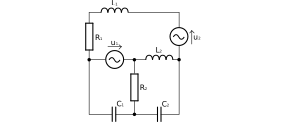
\includegraphics[width=0.8\columnwidth,keepaspectratio]{res/u4o1}
\end{center}
\subsection{Riešenie}
V obvode si nakreslíme tri slučky a zostavíme pre ne rovnice:
\begin{center}
  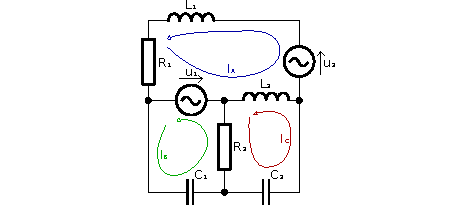
\includegraphics[width=0.8\columnwidth,keepaspectratio]{res/u4o2}
\end{center}
Pre zostavenie rovnice potrebujeme poznať reaktanciu kondenzátora a reaktanciu cievky:
\begin{align*}
    X_C &= \frac{1}{j \omega C} & X_L = j \omega L
\end{align*}
Zostavíme rovnice: 
\begin{flalign*}
    I_A&: I_A\left(j \omega L_1 + R_1 + j \omega L_2\right) - I_C(j \omega L_2) = -U_1 - U_2 &\\
    I_B&: I_B\left(\frac{1}{j \omega C_1} + R_2\right) - I_C R_2 = U_1 \\
    I_C&: I_C\left(R_2 + \frac{1}{j \omega C_2} + j \omega L_2\right) - I_A(j \omega L_2) - I_B{R_2} = 0
\end{flalign*}
$
\begin{pmatrix}
    j \omega L_1 + R_1 + j \omega L_2 & 0 & -j \omega L_2\\
    0 & R_2 + \frac{1}{j \omega C_1} & -R_2 \\
    -j \omega L_2 & -R_2 & R_2 + \frac{1}{j \omega C_2} + j \omega L_2
\end{pmatrix}
\begin{pmatrix}
    I_A \\ I_B \\ I_C
\end{pmatrix}
=
\begin{pmatrix}
    -U_1 - U_2 \\
    U_1 \\
    0
\end{pmatrix}
$ \bigskip \\
Vypočítame sústavu rovníc Cramerovým pravidlom:
\begin{align*}
    \omega = 2 \pi f = 2 \pi 65 = 130 \pi
\end{align*}
$
\begin{pmatrix}
    120 + 102,1j & 0 & -32,67j \\
    0 & 100 - 16,32j & -100 \\
    -32,76i & -100 & 100 + 5,47j
\end{pmatrix}
\begin{pmatrix}
    I_A \\ I_B \\ I_C
\end{pmatrix}
=
\begin{pmatrix}
    -55 \\
    20 \\
    0
\end{pmatrix}
$
\begin{align*}
    D_S = 
    &\begin{vmatrix}
    120 + 102,1j & 0 & -32,67j \\
    0 & 100 - 16,32j & -100 \\
    -32,67j & -100 & 100 + 5,47j
    \end{vmatrix}
    = (120 + 102,1j).(100 - 16,32j).(100 + 5,47j) \\
    & - (-32,67j + 5,47j).(100 - 16,32j).(-32,67j) - (-100).(-100).(120 + 102,1j) = \\
    =& 2,2831 \times 10^{5} - 1.386j \times 10^{5} \\
    D_A = 
    &\begin{vmatrix}
    -55 & 0 & -32,67j \\
    20 & 100 - 16,32j & -100 \\
    0 & -100 & 100 + 5,47j
    \end{vmatrix}
    = (-55).(100 - 16,32j).(100 + 5,47j) \\
    &+ (-32,67j).(20).(-100) - (-100).(-100).(-55) = -4.9079 \times 10^3 + 1.2506j \times 10^5 \\
    D_B = 
    &\begin{vmatrix}
    120 + 102,1j & -55 & -32,67j \\
    0 & 20 & -100 \\
    -32,67j & 0 & 100 + 5,47j
    \end{vmatrix}
    = (120 + 102,1j).(20).(100 + 5,47j) \\
    &+ (-55).(-100).(-32,67j + 5,47j) - (-32,67j + 5,47j).(20).(-32,67j) = \\
    = &2.5019 \times 10^5 + 3.7624j \times 10^4 \\
    D_C = 
    &\begin{vmatrix}
    120 + 102,1j & 0 & -55 \\
    0 & 100 - 16,32j & 20 \\
    -32,67j & -100 & 0 
    \end{vmatrix}
    = -(-32,67j).(100 - 16,32j).(-55) \\
    &- (-100).(20).(120 + 102,1j) = 2.1067 \times 10^5 + 2.4504j \times 10^4 
\end{align*}
Z determinantov vypočítame jednotlivé prúdy: 
\begin{align*}
    I_A = & \frac{D_A}{D_S} = \frac{-4.9079 \times 10^3 + 1.2506j \times 10^5}{2,2831 \times 10^{5} - 1.386j \times 10^{5}} = -0.25869 + 0.39072i~A\\
    I_B = & \frac{D_B}{D_S} = \frac{2.5019 \times 10^5 + 3.7624j \times 10^4}{2,2831 \times 10^{5} - 1.386j \times 10^{5}} = 0.72763 + 0.60651i~A \\
    I_C = & \frac{D_C}{D_S} = \frac{2.1067 \times 10^5 + 2.4504j \times 10^4}{2,2831 \times 10^{5} - 1.386j \times 10^{5}} = 0.62664 + 0.48774i~A
\end{align*}
Vypočítame napätie $U_{C2}$ a $|U_{C2}|$:
\begin{align*}
    &I_{C2} =  I_C \\
    &U_{C2} = X_{C2} . I_{C2} = \frac{1}{j \omega C_2} I_{C2} = \frac{0.627 + 0.488j}{130 \pi j 9 \times 10^{-5}} = 13.269 - 17.048j~V \\ 
    &|U_{C2}| =  \sqrt{13.269 +(-17.048j)^2} = 21.6037~V
\end{align*}
Vypočítame fázový posuv $ \varphi_{C2}$ z napätia $U_{C2}$:
\begin{align*}
    \varphi_{C2} = arctan \left( \frac{Im(U_{C2})}{Re(U_{C2})} \right) = arctan \left( \frac{-17.048}{13.269} \right) = -0,9094~rad = 127^\circ~53'~42,38''
\end{align*}

%     Vypocet determinantov
%     (120+102,1i)*(100-16,32i)*(100+5,47i)-(-32,67i+5,47i)*(100-16,32i)*(-32,67i)-(-100)*(-100)*(120+102,1i)
%     (-55)*(100-16,32i)*(100+5,47i)+(-32,67i)*(20)*(-100)-(-100)*(-100)*(-55)
%     (120+102,1i)*(20)*(100+5,47i)+(-55)*(-100)*(-32,67i+5,47i)-(-32,67i+5,47i)*(20)*(-32,67i)
%     -(-32,67i)*(100-16,32i)*(-55)-(-100)*(20)*(120+102,1i)

\newpage 
